\section{润湿作用}


\begin{frame}
    \frametitle{润湿现象}

    水滴在洁净的玻璃表面上，会铺展成一薄层而不是以滴状形式存在，水滴在植物叶面上则很少铺开。汞滴在玻璃表面上，则主要以滴状形式存在。

    当液体与固体接触时，液体能在固体表面上铺开，即原来的气-固界面被液-固界面代替的过程称为润湿。根据液体对固体润湿情况不同，可分三种情况。
    \begin{itemize}
        \item 沾湿 \quad $W_\mathrm{a} = \Delta G = \sigma_{\mathrm{l-s}} - \sigma_{\mathrm{g-s}} -\sigma_{\mathrm{g-l}}$
        \item 浸湿 \quad $W_\mathrm{i} = \Delta G = \sigma_{\mathrm{l-s}} - \sigma_{\mathrm{g-s}}$
        \item 铺展 \quad $S = \Delta G = \sigma_{\mathrm{g-l}} + \sigma_{\mathrm{l-s}} -\sigma_{\mathrm{g-s}}$
    \end{itemize}

    \begin{figure}[htpb]
        \centering
        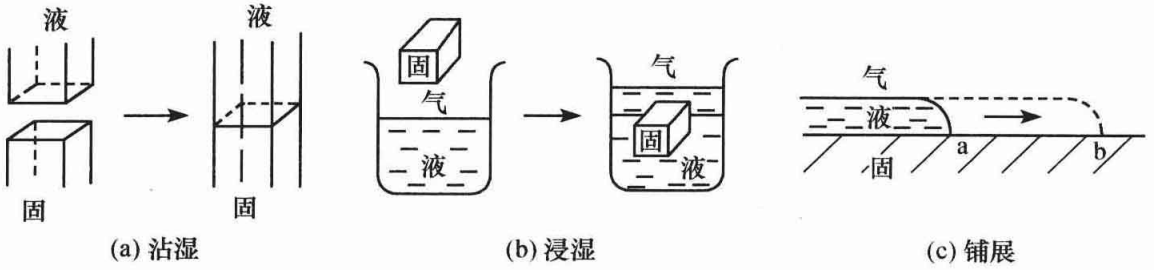
\includegraphics[width=.6\linewidth]{figures/fig8.17.png}
    \end{figure}

\end{frame}


\begin{frame}
    \frametitle{接触角与润湿作用}

    设液体在固体表面上形成液滴，达到平衡时，液滴呈现一定的形状。
    \begin{figure}[htpb]
        \centering
        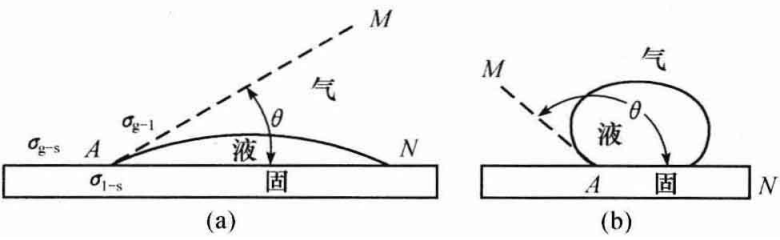
\includegraphics[width=.6\linewidth]{figures/fig8.18.png}
    \end{figure}
    $\theta$称为接触角或润湿角，大小与三种界面张力的相对大小有关，可用实验测定。

    在A点受到三种界面张力的相互作用，气-固界面张力力图使液滴沿固体表面$NA$铺开，遮盖固体表面；气-液界面张力和液-固界面张力则力图使液滴收缩，当达到平衡时，A点受合力为零，因此有
    \[
        \sigma_{\mathrm{g-s}} = \sigma_{\mathrm{l-s}} + \sigma_{\mathrm{g-l}} \cos \theta
    \]

\end{frame}


\begin{frame}
    \frametitle{接触角与润湿作用}
    \[
        \cos \theta = \frac{\sigma_{\mathrm{g-s}} - \sigma_{\mathrm{l-s}}}{\sigma_{\mathrm{g-l}}}
    \]
    上式称为杨氏（Young）方程，它是描述润湿过程的基本方程。
    \begin{itemize}
        \item 如果$\sigma_{\mathrm{g-s}} - \sigma_{\mathrm{l-s}} = \sigma_{\mathrm{g-l}}$，则$\cos \theta=1$，$\theta = 0$，这是完全润湿的情况
        \item 如果$\sigma_{\mathrm{g-s}} - \sigma_{\mathrm{l-s}} < \sigma_{\mathrm{g-l}}$，则$0<\cos \theta<1$，$\theta < 90^{\circ}$，这时固体能被液体润湿
        \item 如果$\sigma_{\mathrm{g-s}} - \sigma_{\mathrm{l-s}} > \sigma_{\mathrm{g-l}}$，则$\cos \theta<0$，$\theta > 90^{\circ}$，这时固体不能被液体润湿
    \end{itemize}
    \[
        \begin{cases}
            W_\mathrm{a} = - \sigma_{\mathrm{g-l}} (1 + \cos \theta) \\
            W_\mathrm{i} = - \sigma_{\mathrm{g-l}} (\cos \theta) \\
            S = \sigma_{\mathrm{g-l}}(1 - \cos \theta)
        \end{cases}
    \]

\end{frame}


\begin{frame}[t]
    \frametitle{}

    \begin{example}
        已知水-石墨体系的下述数据：在298K时，水的表面张力$\sigma_{\mathrm{g-l}} = \SI{0.072}{N.m^{-1}}$，测得水与石墨的接触角为90°。求水与石墨的黏附功、浸湿功和铺展系数。
    \end{example}

\end{frame}


\begin{frame}[t]
    \frametitle{}

    \begin{example}
        293K时，水的表面张力为$\SI{0.072}{N.m^{-1}}$，汞的表面张力为$\SI{0.483}{N.m^{-1}}$，而汞和水的界面张力为$\SI{0.373}{N.m^{-1}}$，试判断（1）水能否在汞的表面上铺展开；（2）汞能否在水的表面上铺展开。
    \end{example}

\end{frame}